\begin{figure}
  \centering
  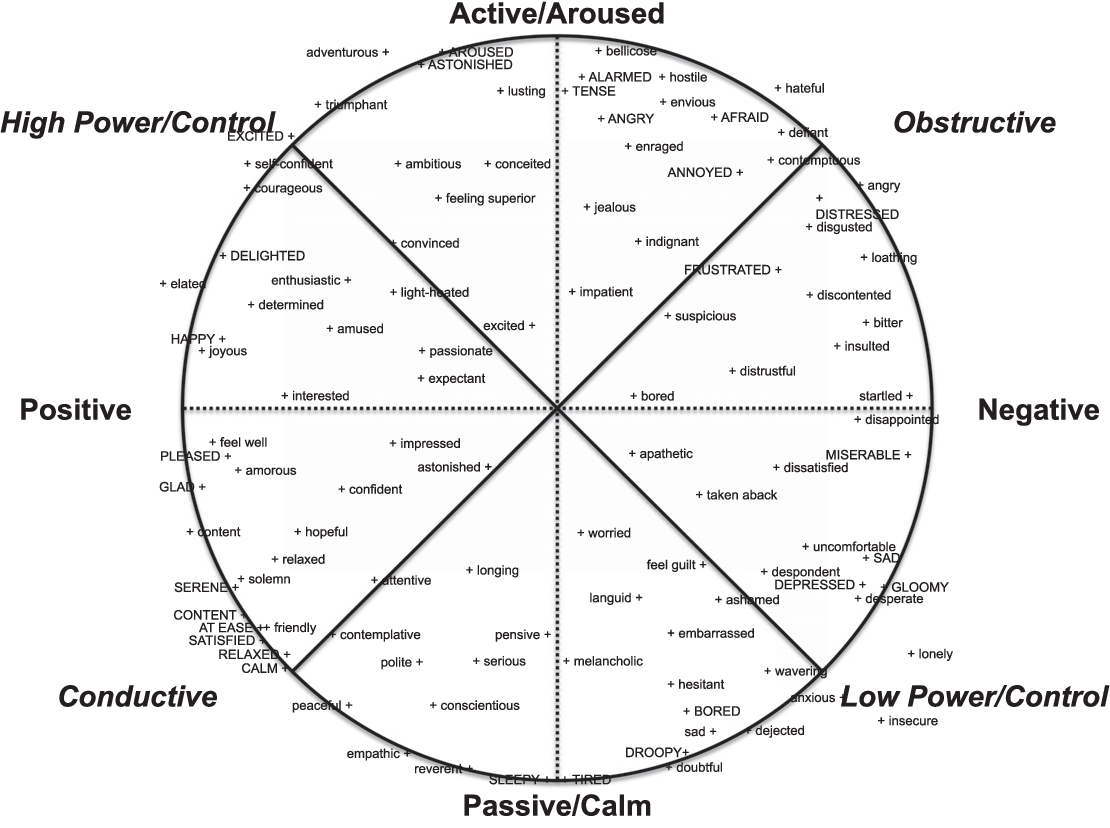
\includegraphics[width=14cm]{./Chapitre1/figures/Genova.png}
  \caption{La roue des émotions de Genève définie par Scherer~\cite{Scherer2005}, qui nomme des émotions (primaires ou secondaires) dans des dimensions continues. On voit par exemple qu'une émotion de valence négative et d'activation passive peut être décrite comme de la fatigue.}
  \label{fig:Genova}
\end{figure}
